\begin{minipage}{0.75\linewidth}
\begin{figure}[h]
    \centering
    \begin{adjustbox}{max width=1.0\linewidth, keepaspectratio}
        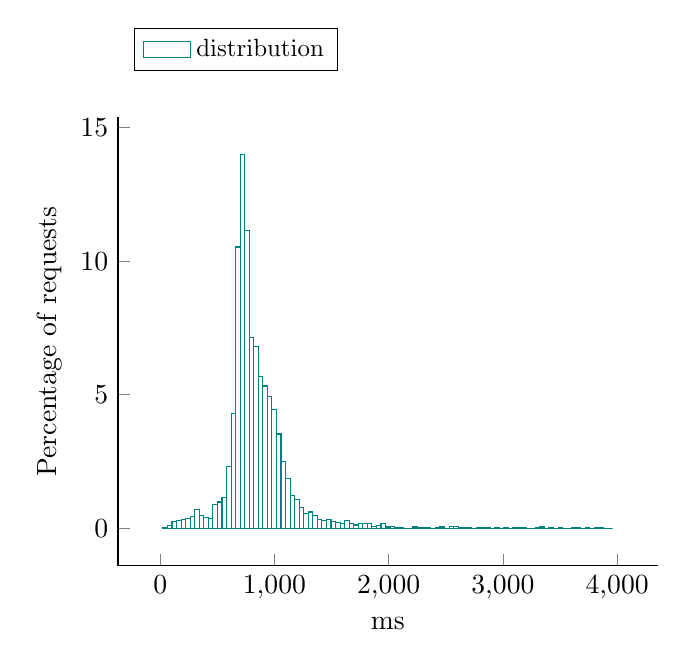
\begin{tikzpicture}
            \begin{axis}[ylabel = Percentage of requests, 
xlabel = ms, 
legend style = {nodes={scale=0.9, transform shape}, at={(0.03,1.2)}, anchor=north west, draw=black, fill=white, align=left, legend columns=3},
area style, mark size = 0pt,
 cycle list name = exotic,
  axis lines* = left]
		\addplot +[ybar interval] coordinates {
			 (24, 0.03125)
			 (63.76, 0.109375)
			 (103.52, 0.265625)
			 (143.28, 0.296875)
			 (183.04, 0.328125)
			 (222.8, 0.375)
			 (262.56, 0.4375)
			 (302.32, 0.703125)
			 (342.08, 0.484375)
			 (381.84, 0.40625)
			 (421.6, 0.359375)
			 (461.36, 0.875)
			 (501.12, 0.984375)
			 (540.88, 1.14062)
			 (580.64, 2.29688)
			 (620.4, 4.3125)
			 (660.16, 10.5312)
			 (699.92, 13.9844)
			 (739.68, 11.1562)
			 (779.44, 7.125)
			 (819.2, 6.79687)
			 (858.96, 5.67188)
			 (898.72, 5.32812)
			 (938.48, 4.9375)
			 (978.24, 4.4375)
			 (1018, 3.53125)
			 (1057.76, 2.48438)
			 (1097.52, 1.875)
			 (1137.28, 1.21875)
			 (1177.04, 1.07812)
			 (1216.8, 0.78125)
			 (1256.56, 0.546875)
			 (1296.32, 0.609375)
			 (1336.08, 0.46875)
			 (1375.84, 0.3125)
			 (1415.6, 0.296875)
			 (1455.36, 0.34375)
			 (1495.12, 0.25)
			 (1534.88, 0.21875)
			 (1574.64, 0.171875)
			 (1614.4, 0.28125)
			 (1654.16, 0.171875)
			 (1693.92, 0.125)
			 (1733.68, 0.1875)
			 (1773.44, 0.171875)
			 (1813.2, 0.171875)
			 (1852.96, 0.078125)
			 (1892.72, 0.09375)
			 (1932.48, 0.1875)
			 (1972.24, 0.046875)
			 (2012, 0.0625)
			 (2051.76, 0.03125)
			 (2091.52, 0.03125)
			 (2131.28, 0)
			 (2171.04, 0)
			 (2210.8, 0.046875)
			 (2250.56, 0.015625)
			 (2290.32, 0.03125)
			 (2330.08, 0.03125)
			 (2369.84, 0)
			 (2409.6, 0.03125)
			 (2449.36, 0.046875)
			 (2489.12, 0)
			 (2528.88, 0.0625)
			 (2568.64, 0.078125)
			 (2608.4, 0.015625)
			 (2648.16, 0.015625)
			 (2687.92, 0.015625)
			 (2727.68, 0)
			 (2767.44, 0.03125)
			 (2807.2, 0.015625)
			 (2846.96, 0.015625)
			 (2886.72, 0)
			 (2926.48, 0.03125)
			 (2966.24, 0)
			 (3006, 0.03125)
			 (3045.76, 0)
			 (3085.52, 0.03125)
			 (3125.28, 0.015625)
			 (3165.04, 0.015625)
			 (3204.8, 0)
			 (3244.56, 0)
			 (3284.32, 0.015625)
			 (3324.08, 0.046875)
			 (3363.84, 0)
			 (3403.6, 0.03125)
			 (3443.36, 0)
			 (3483.12, 0.015625)
			 (3522.88, 0)
			 (3562.64, 0)
			 (3602.4, 0.015625)
			 (3642.16, 0.015625)
			 (3681.92, 0)
			 (3721.68, 0.015625)
			 (3761.44, 0)
			 (3801.2, 0.03125)
			 (3840.96, 0.015625)
			 (3880.72, 0)
			 (3920.48, 0)
			 (3960.24, 0)
		};
\addlegendentry{distribution};
           \end{axis}
      \end{tikzpicture}
  \end{adjustbox}
  \caption{Response time distribution - req = ReadTimeline-2}
\end{figure}
\end{minipage}\hfill\begin{minipage}{0.18\linewidth}
\begin{table}[h]
\begin{tabular}{|cc|}
\hline
\textbf{} & \textbf{ms}\\ \hline
 \Xhline{0.005\arrayrulewidth}
min & 24\\
 \Xhline{0.005\arrayrulewidth}
max & 4000\\
 \Xhline{0.005\arrayrulewidth}
mean & 848\\
 \Xhline{0.005\arrayrulewidth}
std & 308\\
\hline
\hline
 \Xhline{0.005\arrayrulewidth}
25th & 703\\
 \Xhline{0.005\arrayrulewidth}
50th & 784\\
 \Xhline{0.005\arrayrulewidth}
75th & 946\\
 \Xhline{0.005\arrayrulewidth}
80th & 986\\
 \Xhline{0.005\arrayrulewidth}
85th & 1036\\
 \Xhline{0.005\arrayrulewidth}
90th & 1115\\
 \Xhline{0.005\arrayrulewidth}
95th & 1305\\
 \Xhline{0.005\arrayrulewidth}
99th & 1959\\
\hline
\end{tabular}
\caption{Response time}
\end{table}
\end{minipage}\hfill